\documentclass[12pt]{article}
\usepackage{xcolor}
\usepackage{mathtools} % for Figure
\usepackage{wrapfig}
\usepackage[font=small,labelfont=bf]{caption} % make captions of figures smaller and bolded

\usepackage{hyperref}
\hypersetup{
     colorlinks=true,
     linkcolor=blue,
     filecolor=blue,
     citecolor = orange,
     urlcolor=cyan,
}

\usepackage{biblatex}
\addbibresource{ex1_ref.bib}
\renewcommand*{\bibfont}{\normalfont\small} % make references the same size as text

\usepackage[a4paper,
 left=15mm,
 right=15mm,
 bottom=20mm,
 top=15mm]{geometry}

\title{What about the wildlife?}
\author{Enik\H{o} Kevi}
\date{$30^{th}$ of February 2024}

\begin{document}

\maketitle

\textit{"Human activities, principally through emissions of greenhouse gases, have unequivocally caused global warming, with global surface temperature reaching 1.1°C above 1850–1900 in 2011–2020. Global greenhouse gas emissions have continued to increase, with unequal historical and ongoing contributions arising from unsustainable energy use, land use and land-use change, lifestyles and patterns of consumption and production across regions, between and within countries, and among individuals (high confidence)."} \cite{IPCC-Headline}

\section{Introduction}

\begin{wrapfigure}{r}{0.4\textwidth}
    \vspace{-18pt}
    \centering
    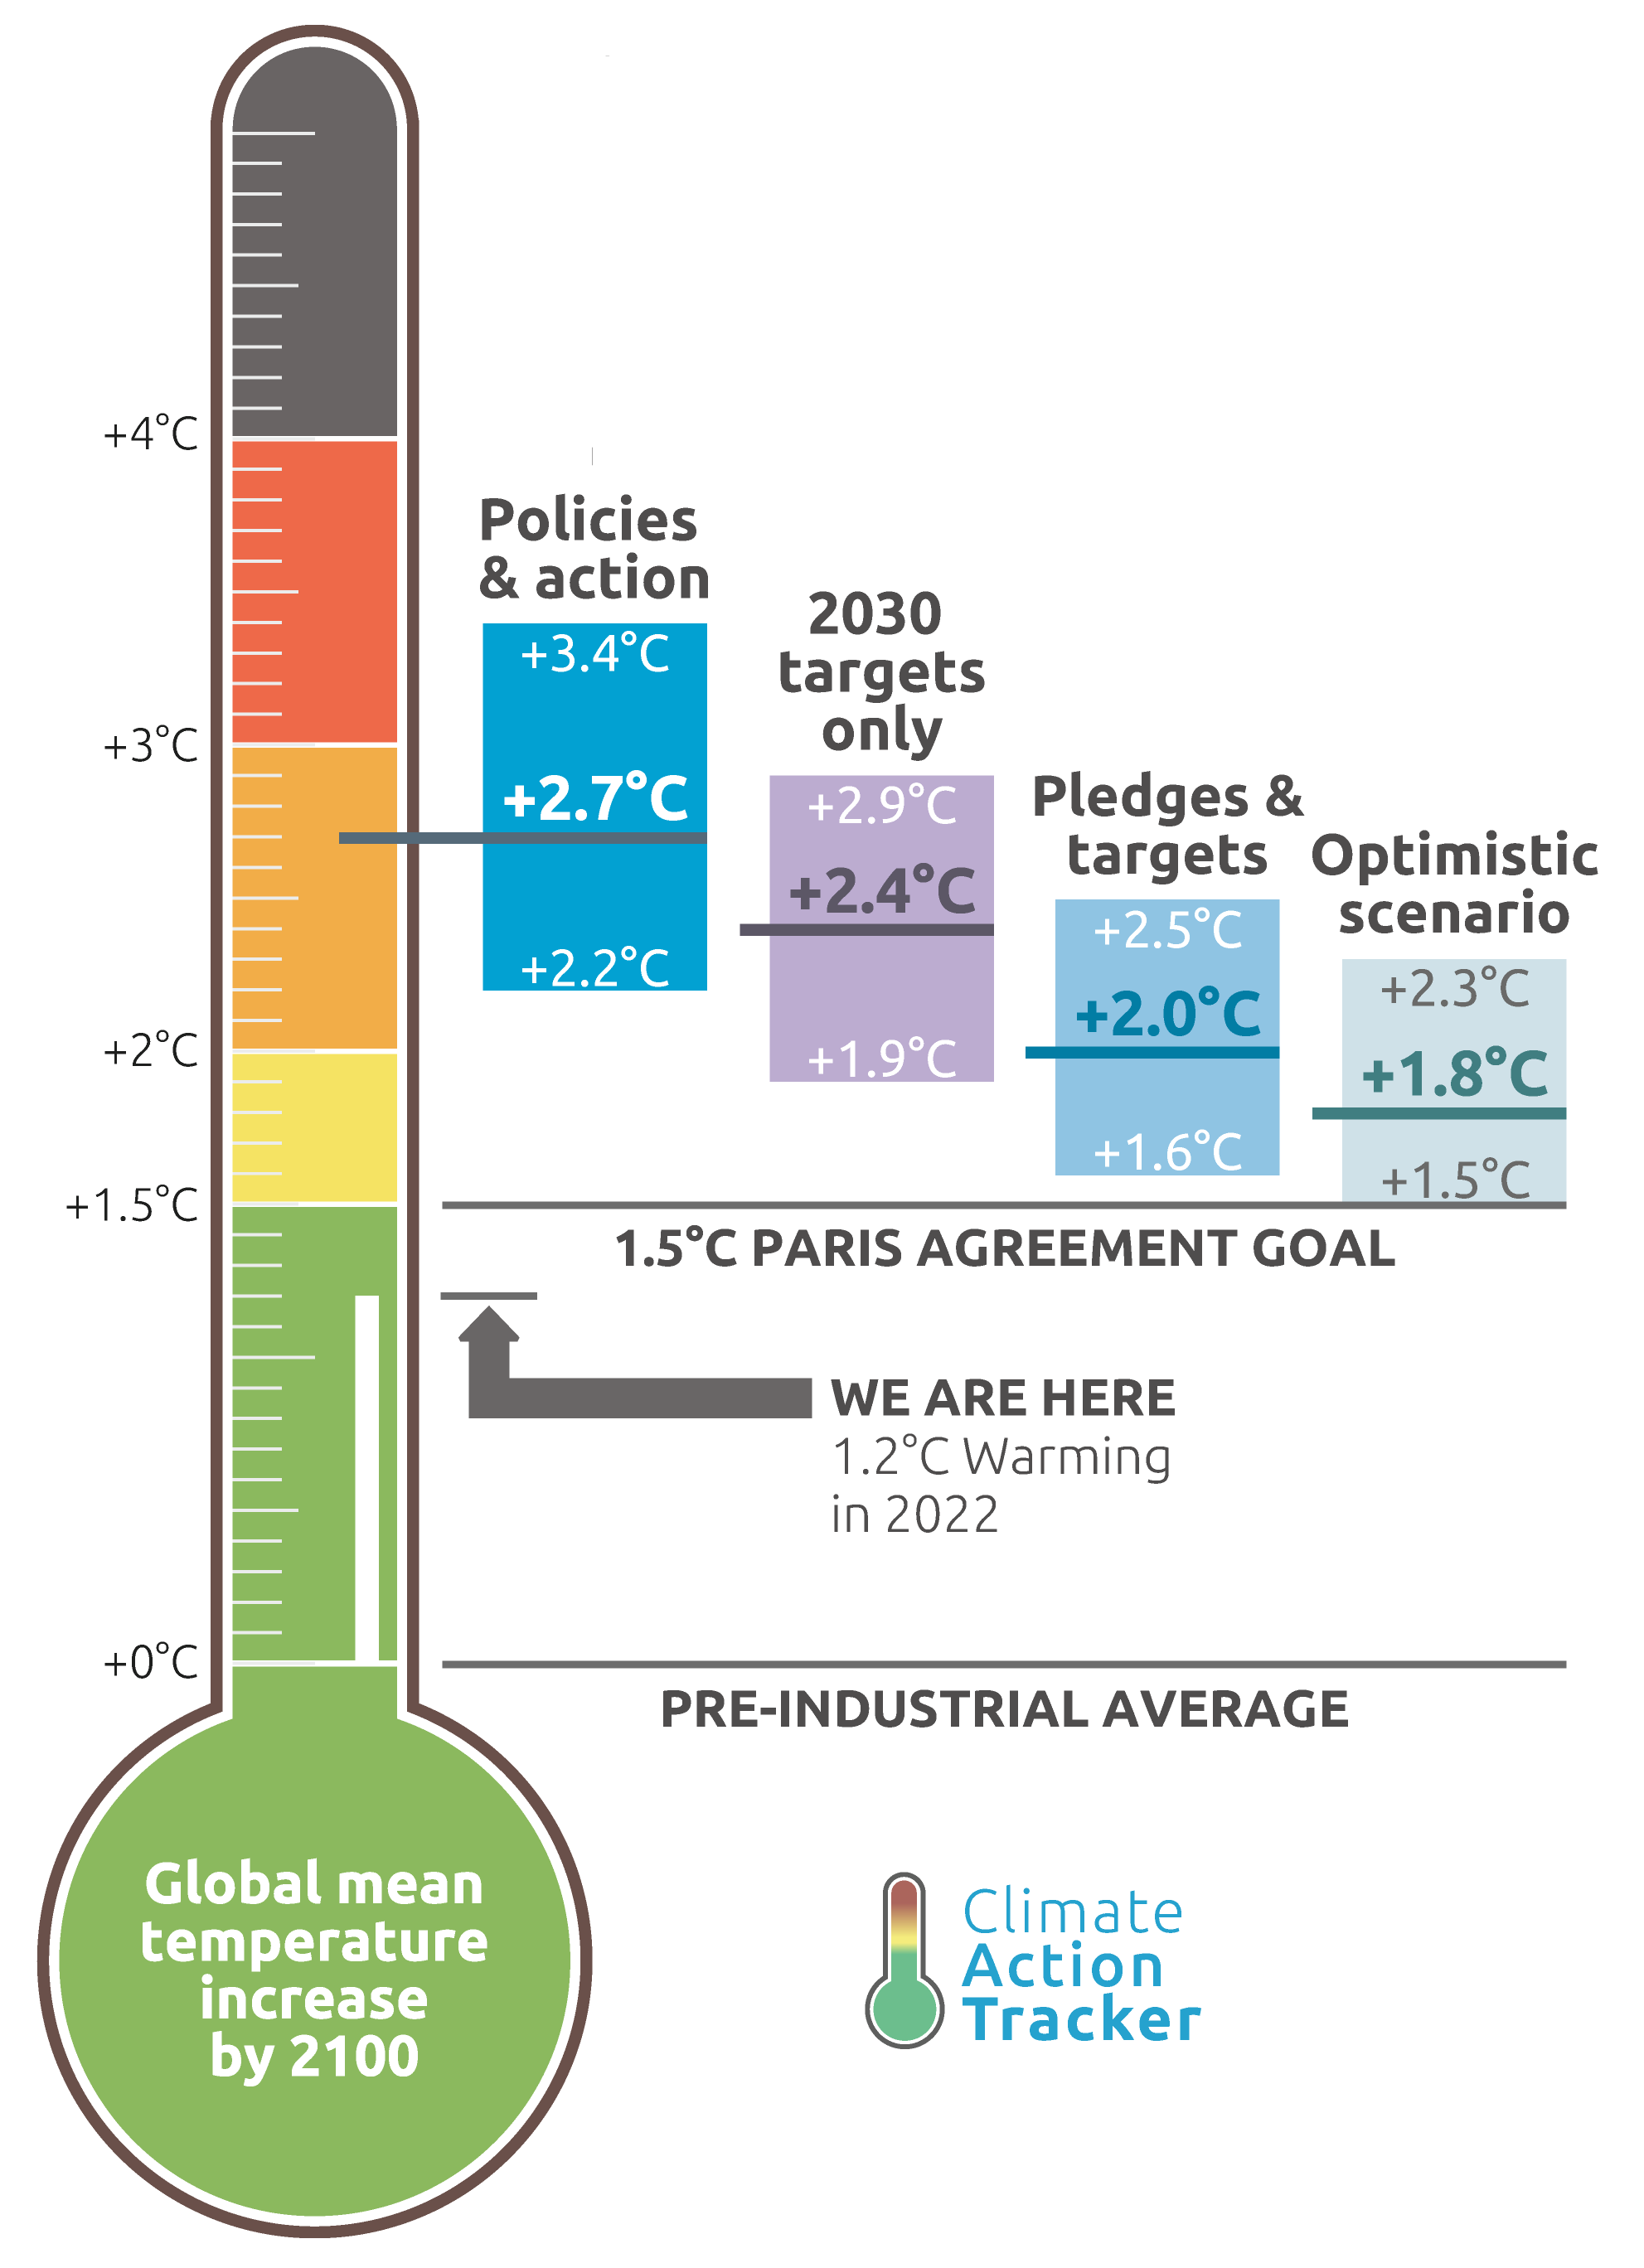
\includegraphics[width=0.78\linewidth]{Figures/cat.png}
    \caption{Global temperature increase by 2100 (for more details visit: \cite{CAT})}
    \label{fig:cat}
\end{wrapfigure}

Reducing human-induced global climate change is one of the biggest challenges of our modern society. While many nations pledge to lessen (or eliminate) their greenhouse gas emissions, the promised policies are slow to implement, and {\color{red} the Earth's temperature rises}. (See the global temperature increase estimation by 2100 on Figure~\ref{fig:cat}.) Global efforts, such as the Intergovernmental Panel on Climate Change (IPCC), have improved our understanding of future climate scenarios over the last decade. Regardless, public opinion toward the severity of climate change remains divided. People with an optimistic mindset tend to think that technological advancements (which \textbf{caused} climate change) will ensure not only the survival of humanity but also our level of comfort in life. However, humans are not alone on planet Earth! Our ability to create and use complex tools is \emph{unique} in the animal kingdom, meaning other species have no means to combat the rapid change in their environment.


\section{Biodiversity and climate change}

\subsection*{Current state}
Scientists expect the global temperature to rise further, even in the most optimistic scenarios. Nevertheless, the current warmer climate already devastates nature, causing frequent wildfires, floods, droughts, coral reef bleaching, and melting ice caps. These environmental changes endanger the local wildlife. These environmental changes endanger the local wildlife and risk species extinction. (An interesting personal testimony is \href{https://en.wikipedia.org/wiki/David_Attenborough:_A_Life_on_Our_Planet}{David Attenborough: A Life on Our Planet} both in book or film format.)

\subsection*{Future scenarios}

As the global climate warms, the environmental impacts get more acute. Besides the impact on food production, many species may lose their habitat entirely. Figure~\ref{fig:wildlife} estimates the biodiversity loss with different climate scenarios. Comparing Figure~\ref{fig:wildlife} with the previous Figure~\ref{fig:cat} we see how even realistic scenarios result in massive wildlife loss worldwide.

\begin{figure}[!h]
    \centering
    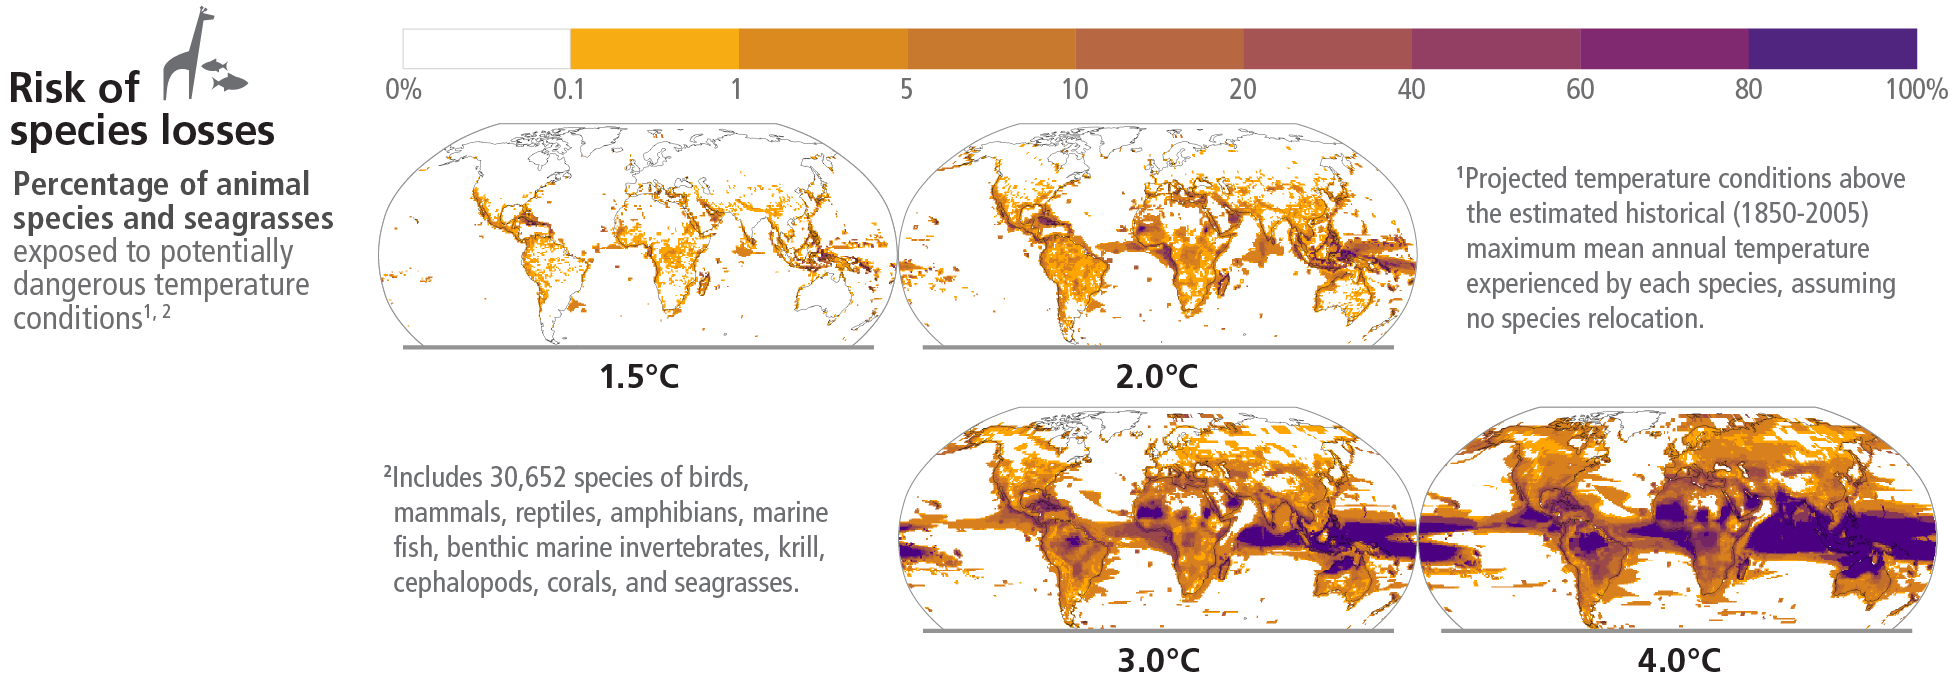
\includegraphics[width=\linewidth]{Figures/wildlife-loss.png}
    \caption{Projected risks and impacts of climate change on natural systems at different global warming levels relative to 1850–1900 levels. \cite{IPCC-Wildlife-Figure}}
    \label{fig:wildlife}
\end{figure}

\section{Personal solutions}

When we look at the global greenhouse emissions per sector (see Figure~\ref{fig:ghg-sector}), it is easy to think that the key players of pollution are industries, multinational companies, governments, etc. These figures mask the contribution of individuals and show it on a societal level. However, everyone is part of society, and small personal changes can create a drastic difference if enough people decide to change. For example, one can:

\begin{itemize}
    \setlength\itemsep{1pt}
    \item investigate which aspect of life one could change to be more environmentally friendly
    \item reduce traveling by plane
    \item commute by bike or on foot
    \item reduce meat consumption (especially beef)
    \item avoid buying new products (cars, phones, computers, clothes, furniture, etc.)
    \item buy local products (less pollution from transportation, etc.)
    \item vote for politicians who care about climate change
    \item raise awareness around you and motivate people to change
\end{itemize}

\section{Conclusion}

Life may be easy, life may be hard. We may blame others or stay in blissful ignorance. Nevertheless, we are all on Earth and share its resources, bounties, and shortages. Pose, ponder, prioritize, and act!

\clearpage

\begin{figure}
    \centering
    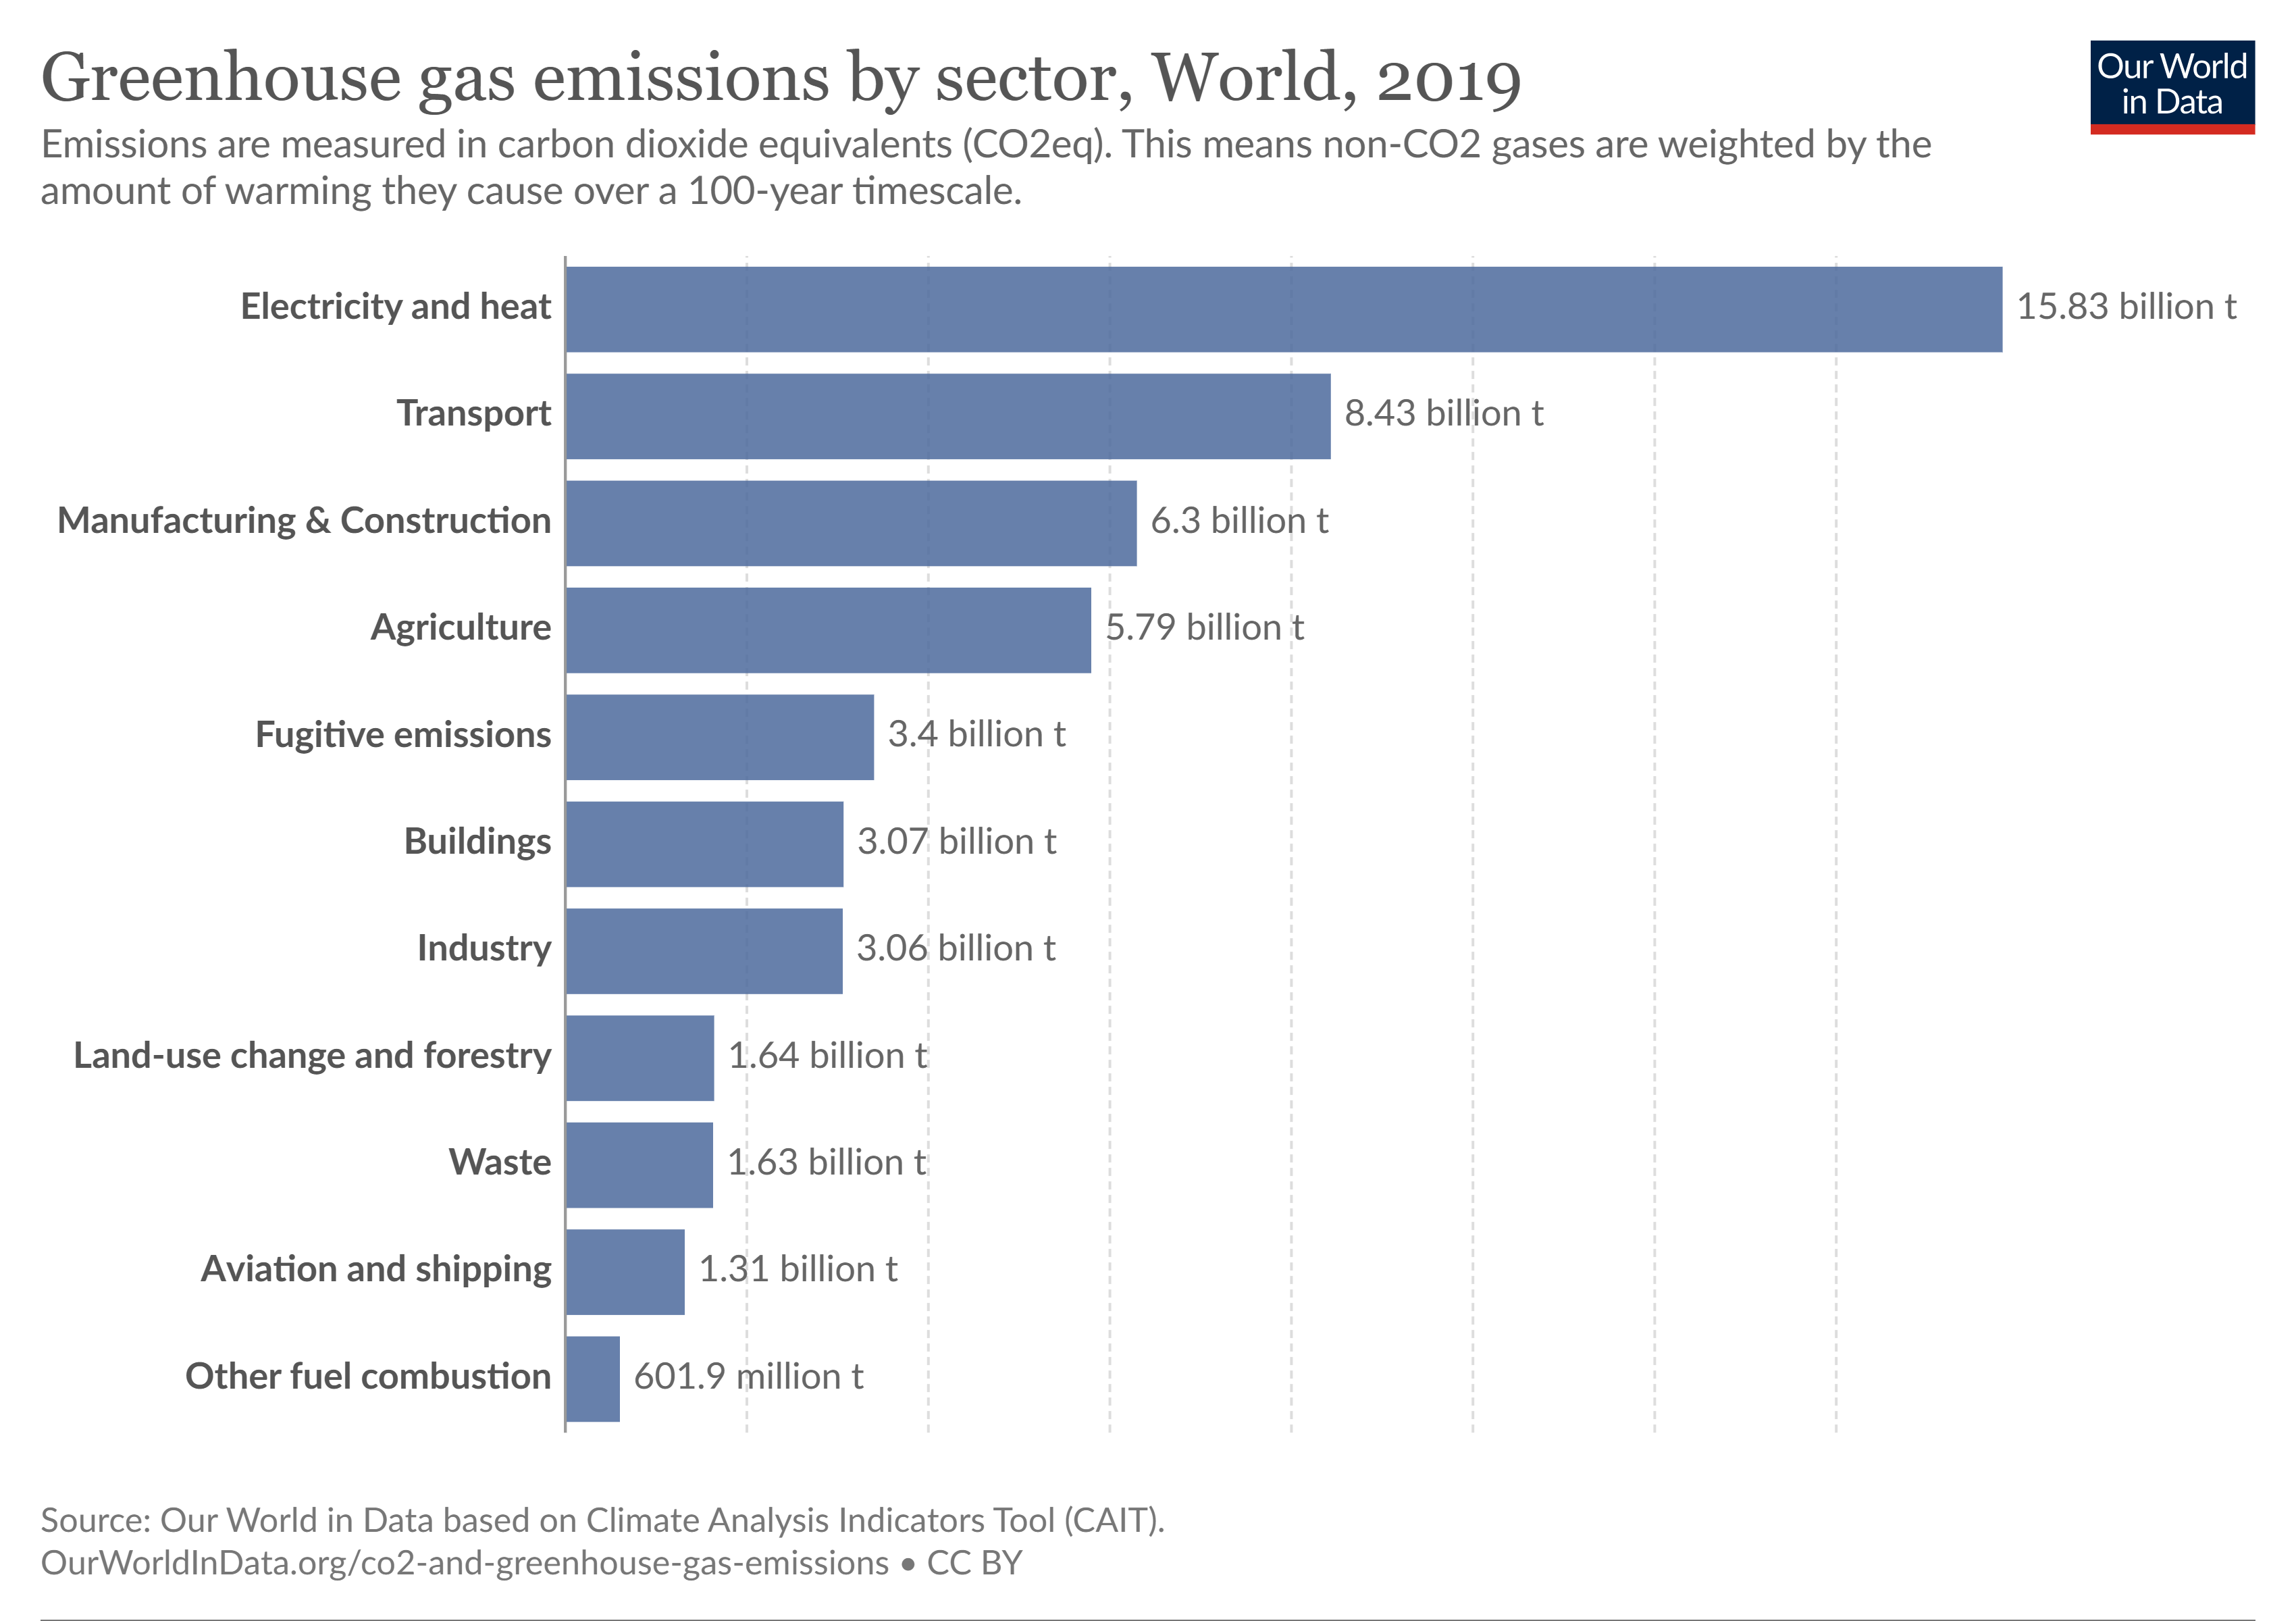
\includegraphics[width=\linewidth]{Figures/ghg-emissions-by-sector.png}
    \caption{Greenhouse gas emissions by sector in the world in 2019 \cite{GHG-Sector}}
    \label{fig:ghg-sector}
\end{figure}

\printbibliography

\end{document}
